\documentclass[xcolor=pdftex,dvipsnames,table,aspectratio=169]{beamer}
%\documentclass[xcolor=pdftex,dvipsnames,table,handout,aspectratio=169]{beamer}

%\setbeameroption{show notes}

\usepackage{bm,graphicx,multirow,amsmath,tikz} %fancybox,
\usepackage{color}%,textpos}
\usepackage[round]{natbib}
\usepackage[normalem]{ulem}
\usepackage{hyperref}
\usepackage{lastpage}
\usepackage{array}
\usepackage{color}
\usepackage{framed}
\usepackage{hyperref}

% Define Western colours
\definecolor{western}{rgb}{.306,.152,.524}
\definecolor{westerngray}{rgb}{.512,.508,.524}

%% Define BEAMER colours
\setbeamercolor{frametitle}{bg=western,fg=white}
\setbeamercolor{framesubtitle}{bg=western,fg=black}
\setbeamercolor{title}{fg=white,bg=western}
\setbeamercolor{author}{fg=white,bg=western}
\setbeamercolor{institute}{fg=white,bg=western}
\setbeamercolor{date}{fg=white,bg=western}

%% Set BEAMER fonts
\setbeamerfont{title}{shape=\bf}
\setbeamerfont{frametitle}{shape=\sc,size=\Large}
\setbeamerfont{framesubtitle}{shape=\sc,size=\Large}
\setbeamerfont{footline}{shape=\sc}

%% Define BEAMER toc
\setbeamercolor{section in toc}{fg=western}
\setbeamercolor{subsection in toc}{fg=westerngray}
\setbeamertemplate{sections/subsections in toc}[ball]

%% Define BEAMER background
\setbeamercolor{background canvas}{bg=white}

%% Define BEAMER footer
\setbeamertemplate{navigation symbols}{}
\setbeamercolor{footline}{fg=white,bg=western}
\setbeamertemplate{footline}{%
  \begin{beamercolorbox}[wd=\paperwidth]{footline}
    \vskip5pt

    \raisebox{.05in}{
      \scriptsize{\bf \insertshorttitle}
    }
    \hfill
    \raisebox{.05in}{
      \scriptsize{\bf \insertframenumber/\inserttotalframenumber} 
    }
    \hspace{5pt}

    \vskip5pt
  \end{beamercolorbox}
}

%% Define BLOCK environment
\setbeamercolor{block title}{fg=western}
\setbeamerfont{block title}{series=\bfseries}

%% Define ENUMERATE and ITEMIZE environements
\setbeamertemplate{itemize item}[ball]
\setbeamertemplate{enumerate item}[ball]
\setbeamercolor{item projected}{bg=western}

%% Define BEAMER toc
\setbeamercolor{sections/subsections in toc}{fg=blue!75}
\setbeamertemplate{sections/subsections in toc}[ball]

% %% Define SECTION openings
% \AtBeginSection[]{
%   \begin{frame}{\insertshorttitle}
%     \tableofcontents[currentsection,subsectionstyle=hide/hide/hide]
    
%   \end{frame}
% }

%% Define BEAMER frametitle
\addtobeamertemplate{frametitle}{
   \let\insertframetitle\insertsectionhead}{}
\addtobeamertemplate{frametitle}{
   \let\insertframesubtitle\insertsubsectionhead}{}


\makeatletter
  \CheckCommand*\beamer@checkframetitle{\@ifnextchar\bgroup\beamer@inlineframetitle{}}
  \renewcommand*\beamer@checkframetitle{\global\let\beamer@frametitle\relax\@ifnextchar\bgroup\beamer@inlineframetitle{}}
\makeatother

% Define counters for example and exercise
\newcounter{example}
\newcounter{exercise}

% Define example and exercise commands
\renewcommand{\example}
{\stepcounter{example}Example \lecturenum.\arabic{example}}
\newcommand{\examplectd}
{Example \lecturenum.\arabic{example}\ ctd}
\newcommand{\exercise}
{\stepcounter{exercise}Exercise \lecturenum.\arabic{exercise}}
\newcommand{\exercisectd}
{Exercise \lecturenum.\arabic{exercise}\ ctd}

\usepackage{enumitem}

\newcommand{\lecturenum}{10}

\title[SS2857]{Probability and Statistics I}
\subtitle{\lecturenum. The Binomial Probability Distribution}

\date{}

%% Add logo
% \titlegraphic{\includegraphics[height=2cm]{../uwo_logo_reversed}}

%% Initialize R


\begin{document}

{
\setbeamertemplate{footline}{}
\setbeamercolor{background canvas}{bg=western}

\begin{frame}
  \addtocounter{framenumber}{-1}

  \maketitle
\end{frame}
}

\begin{frame}
  \frametitle{\invisible{Hello}}

  \begin{center}
    \Large{\textbf{3.5 The Binomial Probability Distribution}}
  \end{center}

  \begin{center}
    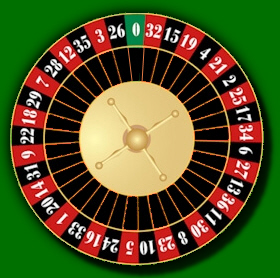
\includegraphics[height=.5\textheight]{roulette_wheel}
  \end{center}

\end{frame}

\begin{frame}

\begin{block}{\example}
What is the probability of each of these events?

\medskip

\begin{enumerate}[label=\alph*),start=1]
\item You toss a fair coin 5 times and it lands heads side up 3 times?
\item You draw 5 cards from a standard deck \textit{with replacemnt} and draw 3 red cards?
\item You guess the answer to 5 true or false questions on a quiz and get three correct.
\item You roll a fair die 5 times and the number shown is odd on 3 rolls. 
\end{enumerate}

\end{block}
\end{frame}

\begin{frame}
  
  \begin{block}{Binomial Experiment}
    An experiment is a binomial experiment if
    \begin{enumerate}[label=\alph*),start=1]
    \item It consists of a fixed number of $n$ trials.
    \item Each trial can result in two outcomes (success and failure).
    \item The trials are mutually independent.
    \item The probability of success is on each trial a constant, denoted by $p$.
    \end{enumerate}
  \end{block}
  
\end{frame}

\section{The Binomial Distribution}

\begin{frame}

  \begin{block}{\example: The Binomial Experiment}
    Approximately 79\% of the world's population has brown eyes \footnote{\url{https://www.worldatlas.com}}.
    
    Suppose that we sample 5 people from the population at random and record their eye-colour as brown or not brown. Let $X$ represent the number of people in our sample with brown eyes.
    
    \bigskip

    \begin{center}
      Is this a binomial experiment?
    \end{center}
  \end{block}
  
\end{frame}


\begin{frame}
  \begin{block}{Binomial Random Variables}
    Let $X$ count the number of successes in a binomial experiment with $n$ trials and probability of success $p$.

    \bigskip
    
    Then $X$ is said to be a binomial random variable. Alternatively, we say that $X$ has a binomial distribution.

    \bigskip

      Mathematically we write
      $$
      X \sim \mbox{Binomial}(n,p).
      $$

  \end{block}
\end{frame}

\begin{frame}
  Suppose that 
   $$
   X \sim \mbox{Binomial}(n,p).
   $$
  
  \begin{block}{PMF and CDF}
    \begin{itemize}
    \item PMF: $b(x;n,p)=\binom{n}{x}p^x(1-p)^{n-x},\quad x=0,\ldots,n$
    \item CDF: requires special functions
    \end{itemize}
  \end{block}
  
  \begin{block}{Properties}
    \begin{itemize}
    \item Mean: $\mu=np$
    \item Variance: $\sigma^2=np(1-p)$
    %\item Skewness: $E\left[\left(\frac{X-\mu_X}{\sigma_X}\right)^3\right]=\frac{1-2p}{\sqrt{np(1-p)}}=\frac{1-2p}{\sigma}$
    \end{itemize}
  \end{block}
  
    \begin{block}{Calculator}
  \url{https://stattrek.com/online-calculator/binomial}
  \end{block}
\end{frame}

\begin{frame}

  \begin{block}{\example: The Binomial Distribution}
    A standard roulette wheel has 37 pockets in which the ball may land. Of these, 18 pockets are red, 18 are black, and 1 is green.

    \begin{center}
      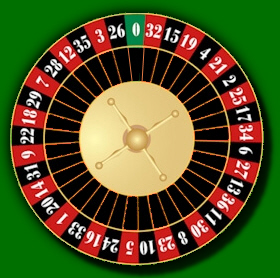
\includegraphics[height=.7\textheight]{roulette_wheel}
    \end{center}
  \end{block}
\end{frame}

\begin{frame}

  \begin{block}{\examplectd: The Binomial Distribution}
    A standard roulette wheel has 37 pockets in which the ball may land. Of these, 18 pockets are red, 18 are black, and 1 is green.

    \bigskip
    
    Suppose that you place \$1 bets that the ball will land in a black pocket on 20 consecutive games. Let $X$ be the number of times you win.

    \begin{enumerate}[label=\alph*),start=1]
    \item Why is this a binomial experiment?
    \item What is the distribution of $X$?
    \item What is the pmf of $X$?
    \item What is the probability that you win exactly half the games?
    \end{enumerate}
  \end{block}
\end{frame}

\begin{frame}

  \begin{block}{\examplectd: The Binomial Distribution}
    A standard roulette wheel has 37 pockets in which the ball may land. Of these, 18 pockets are red, 18 are black, and 1 is green.

    \bigskip
    
    Suppose that you place \$1 bets that the ball will land in a black pocket on 20 consecutive games. Let $X$ be the number of times you win.
    
    \begin{enumerate}[label=\alph*),start=5]
    \item What is the probability that you win more than half the games?
    \item What are the mean, variance, and standard deviation of $X$?
    \item Let \$$v$ be the amount you win on a \$1 bet if the ball lands in a black pocket. What value of \$$v$ makes this a fair game?
    \end{enumerate}
    
  \end{block}
\end{frame}

\begin{frame}

\begin{block}{\exercise}
The shooting percentage in hockey records the percentage of shots on goal taken in a season on which a player scores. The highest shooting percentage in the 2023-2024 NHL season, 24.5\%, was claimed by Sam Reinhart of the Florida Panthers.

Suppose that Sam takes 200 shots on net in the 2024-2025 season with the same shooting percentage. Let $S$ be the number of goals Sam scores. 

\begin{enumerate}[label=\alph*),start=1]
\item Explain why it makes sense to consider this a binomial experiment.
\item State the distribution of $S$.
\item What is the pmf of $S$?
\item What are the expected value and standard deviation of $S$?
\item What is the probability that Sam scores at least than 50 goals?
\end{enumerate}
\end{block}
\end{frame}


\end{document}
